
\documentclass[pdflatex,sn-mathphys-num]{sn-jnl}% Math and Physical Sciences 
\usepackage{graphicx}%
\usepackage{multirow}%
\usepackage{amsmath,amssymb,amsfonts}%
\usepackage{pgfplots}
\usepackage{pgfplotstable}
\usepackage{filecontents}
\pgfplotsset{compat=1.18}
\usepackage{amsthm}%
\usepackage{mathrsfs}%
\usepackage[title]{appendix}%
\usepackage{xcolor}%
\usepackage{textcomp}%
\usepackage{manyfoot}%
\usepackage{booktabs}%
\usepackage{algorithm}%
% \usepackage{algorithm2e}%
\usepackage{algorithmicx}%
\usepackage{algpseudocode}%
\usepackage{url}%
\usepackage{ltxtable}%
\usepackage{tikz}%
\usepackage{float}%
\usepackage{tabularx}%
\usepackage{array}%
\usepackage[utf8]{inputenc}%
% Theorem styles
\theoremstyle{thmstyleone}
\newtheorem{theorem}{Theorem}
\newtheorem{proposition}[theorem]{Proposition}

\theoremstyle{thmstyletwo}
\newtheorem{example}{Example}
\newtheorem{remark}{Remark}

\theoremstyle{thmstylethree}
\newtheorem{definition}{Definition}

\raggedbottom

\begin{document}

\title[Article Title]{\textbf{Detection of Primary User Emulation Attacks in Cognitive Radion Network Using Clustering Approach }}

\author*[1]{\fnm{Nandita} \sur{Louriyam}}\email{lnandita123@gmail.com}

\author[2]{\fnm{Rishav} \sur{Raj}}\email{srishav1911@gmail.com}
\equalcont{These authors contributed equally to this work.}

\author[3]{\fnm{Snehasish} \sur{Das}}\email{snehasish202@gmail.com}
\equalcont{These authors contributed equally to this work.}

\author[4]{\fnm{Sumir} \sur{Das}}\email{sumir123@gmail.com}
\equalcont{These authors contributed equally to this work.}

\author[5]{\fnm{Debraj} \sur{Dutta Gupta}}\email{debraj123@gmail.com}
\equalcont{These authors contributed equally to this work.}

\affil[1,2,3,4,5]{\orgdiv{Computer Science and Engineering}, \orgname{Assam University}, \orgaddress{\street{Silchar}, \city{Silchar}, \postcode{788011}, \state{Assam}, \country{India}}}


\abstract{Primary User Emulation Attacks (PUEA) pose a critical security threat to cognitive radio networks by mimicking legitimate primary user transmissions, leading to spectrum underutilization and network performance degradation. Existing detection methods struggle with varying network topologies and lack robust clustering algorithms capable of handling diverse operational scenarios. This paper proposes an integrated multi-topology PUEA detection system using enhanced clustering algorithms (K-means, Agglomerative, Spectral) with KNN and Means classification refinement techniques. We simulate 75 diverse network topologies across three distance scenarios: far (100 units), medium (65 units), and close (30 units) PU-PUEA separation, with five PUEA activity levels (10\%-50\%). Statistical features (mean, variance, median, quartiles) are extracted from received power measurements across 400 time slots. Results demonstrate that K-means achieves superior detection rates exceeding 97\% at low PUEA activity levels with false detection rates around 21\% in favorable conditions. Spectral clustering shows moderate performance with detection rates of 42-50\%, while Agglomerative clustering achieves detection rates of 30-37\% across different PUEA activity levels. The multi-topology validation framework ensures robust PUEA detection across diverse network conditions, providing practical deployment guidelines for cognitive radio security systems. Our approach advances unsupervised anomaly detection by eliminating the need for labeled training data while maintaining high detection accuracy across varying spatial configurations.}



\keywords{Cognitive Radio, PUEA Detection, Clustering Algorithms, Network Security, Spectrum Sensing, Multi-topology Analysis}


\maketitle

\section{Introduction}\label{sec1}

The exponential growth in wireless communication demand has created unprecedented spectrum scarcity challenges. Cognitive Radio Networks (CRNs) \cite{ref2} emerge as a promising solution through Dynamic Spectrum Access (DSA), enabling secondary users (SUs) to opportunistically utilize unused spectrum bands allocated to primary users (PUs). However, the open and dynamic nature of CRNs introduces significant security vulnerabilities, with Primary User Emulation Attacks (PUEA) representing one of the most critical threats.

In PUEA, malicious nodes transmit signals that mimic legitimate primary user characteristics, deceiving secondary users into vacating spectrum bands unnecessarily. This attack can severely degrade network performance, reduce spectrum efficiency, and compromise the fundamental cognitive radio principle of non-interference with primary users. Existing detection methods rely on cryptographic authentication or supervised learning approaches, which face limitations in practical deployment due to key distribution challenges and the requirement for labeled attack data \cite{ref5,ref9}.

The rapid proliferation of wireless devices and the exponential growth in data traffic demand have intensified the need for efficient spectrum management solutions. Traditional spectrum allocation policies, which assign fixed frequency bands to licensed users, often result in significant spectrum underutilization. Studies indicate that licensed spectrum bands remain unused for substantial periods, creating opportunities for more efficient spectrum sharing mechanisms \cite{ref1}.

Cognitive Radio Networks address this challenge by introducing intelligent spectrum access capabilities. These networks consist of cognitive radio devices capable of sensing their electromagnetic environment, identifying available spectrum opportunities, and adapting their transmission parameters accordingly. The cognitive cycle involves four primary functions: spectrum sensing, spectrum decision, spectrum sharing, and spectrum mobility.

Despite their promising potential, CRNs face numerous security challenges that can compromise their effectiveness and reliability \cite{ref25,ref7}. Among these threats, Primary User Emulation Attacks (PUEA) represent one of the most sophisticated and damaging security vulnerabilities. The impact of PUEA extends beyond immediate spectrum denial, cascading into broader network disruptions, including reduced quality of service, increased latency, and degraded network performance \cite{ref4,ref8}.\\

% \subsection{Research Gaps and Drawbacks of Existing Methods}

Despite extensive research efforts in PUEA detection, existing approaches suffer from several critical limitations and research gaps:

\textbf{Machine Learning Approaches Limitations:} Current machine learning methods for PUEA detection face significant drawbacks including dependency on large labeled datasets for training, poor generalization to unknown attack patterns, and computational complexity that limits real-time deployment. Supervised learning approaches require extensive labeled attack data which is often unavailable in practical scenarios, while deep learning methods suffer from black-box decision making that lacks interpretability for security-critical applications \cite{ref9,ref22}.

\textbf{Energy Detection Method Drawbacks:} Traditional energy detection techniques demonstrate poor performance under low Signal-to-Noise Ratio (SNR) conditions and are highly susceptible to noise uncertainty. These methods cannot differentiate between legitimate primary user signals and sophisticated PUEA attacks that employ similar power levels, leading to high false alarm rates and reduced detection accuracy \cite{ref1,ref11}.

\textbf{Cryptographic Authentication Limitations:} Cryptographic approaches face practical deployment challenges including complex key distribution infrastructure, significant computational overhead for resource-constrained cognitive radio devices, and vulnerability to key compromise attacks. The requirement for secure key management and certificate authorities limits scalability in dynamic cognitive radio environments \cite{ref5,ref6}.

\textbf{Signal Processing Technique Constraints:} Existing signal processing methods require detailed knowledge of legitimate primary user signal characteristics and are vulnerable to sophisticated attackers who can closely mimic these characteristics. These approaches struggle with varying channel conditions and lack robustness against adaptive attack strategies \cite{ref4,ref17}.

\textbf{Clustering-Based Method Inadequacies:} Current clustering approaches for PUEA detection lack systematic performance evaluation across diverse network topologies and suffer from poor parameter selection strategies. Existing methods demonstrate limited effectiveness in handling varying spatial attack scenarios and lack robust post-processing enhancement techniques \cite{ref12,ref13,ref21}.

\subsection{Contributions of This Paper}

To address these critical research gaps, the contributions of this paper are summarized as follows:

1. We propose the first comprehensive multi-topology PUEA detection framework using clustering algorithms validated across 75 diverse network realizations to ensure statistical significance and generalizability.

2. We introduce a size-based heuristic for cluster identification after applying the clustering method that significantly outperforms complex statistical variance methods, providing robust and computationally efficient PUEA detection without requiring detailed primary user signal knowledge.

3. We introduce innovative enhancement methods using K-Nearest Neighbors (KNN) and Means-based refinement algorithms that improve clustering accuracy by 25-35\% without requiring labeled training data, addressing the limitations of supervised learning approaches.

4. We provide the first systematic evaluation of PUEA detection performance across three distinct distance scenarios (far/medium/close), revealing critical vulnerability patterns and spatial dependency relationships that existing literature has not addressed.

5. We employ multiple performance metrics including Detection Rate, False Detection Rate, providing comprehensive assessment beyond traditional binary classification metrics used in existing literature.

\section{Related Work}\label{sec2}

This section provides a comprehensive review of existing PUEA detection literature, categorizing approaches based on their detection methodologies and identifying research gaps that our work addresses. We systematically examine five major categories of PUEA detection techniques: cryptographic and authentication-based methods, signal processing approaches, machine learning techniques, clustering-based detection methods, and cooperative sensing strategies. For each category, we analyze the fundamental principles, strengths, limitations, and practical deployment challenges to establish the foundation for our enhanced clustering framework.

% \subsection{Cryptographic and Authentication Approaches}

Cryptographic approaches authenticate primary user signals through digital signatures and certificates. Liu et al. \cite{ref5} proposed authenticating primary users' signals via integrated cryptographic and wireless link signatures, demonstrating how cryptographic techniques can enhance spectrum sensing security. Jin et al. \cite{ref6,ref15} developed detection methods for primary user emulation attacks in dynamic spectrum access networks, providing both theoretical foundations and practical algorithms.

However, these approaches face key distribution and computational overhead challenges in practical deployments. The requirement for secure key distribution infrastructure and the computational burden of cryptographic operations limit their applicability in resource-constrained cognitive radio devices.

% \subsection{Signal Processing Techniques}

Traditional signal processing approaches analyze physical layer characteristics like signal strength patterns and modulation features. Chen et al. \cite{ref4} proposed one of the foundational defense mechanisms against primary user emulation attacks, focusing on exploiting the unique characteristics of primary user signals to distinguish them from emulated signals. Gupta and Sahu \cite{ref1} provided a comprehensive overview of PUEA detection techniques, emphasizing energy detection and feature-based approaches.

Shah and Sastry \cite{ref11} introduced proactive transmission power control techniques for PUEA detection, demonstrating how adaptive power management can enhance detection accuracy. However, these methods require detailed knowledge of legitimate primary user signal characteristics and may be vulnerable to sophisticated attackers who can closely mimic these characteristics.

% \subsection{Machine Learning Approaches}

Machine learning techniques have gained attention for PUEA detection due to their ability to learn complex attack patterns. Wang et al. \cite{ref9} developed machine learning-based detection methods specifically for PUEA, demonstrating superior performance compared to traditional approaches. Zhao \cite{ref22} proposed a reliable spectrum sensing method based on deep learning for PUEA detection, showing how supervised learning can effectively distinguish between legitimate and emulated signals.

Kim et al. \cite{ref10} investigated deep learning approaches for robust detection in related attack scenarios, while Chhetry and Marchang \cite{ref23} investigated one-class classification methods for PUEA detection, employing advanced anomaly detection techniques. However, supervised methods require extensive labeled datasets and may not generalize well to unknown attack patterns.

% \subsection{Clustering-Based Detection Methods}

Clustering algorithms have gained prominence in PUEA detection due to their ability to identify natural groupings in signal data without requiring labeled training datasets. Taggu and Marchang \cite{ref21} proposed a DBSCAN-based technique for detecting colluding attacks, demonstrating the effectiveness of density-based clustering in wireless security applications.

Luo et al. \cite{ref13} developed novel clustering-based feature extraction methods specifically for PUEA detection, showing how clustering principles can enhance feature discrimination. Singh et al. \cite{ref14} investigated distance-based outlier approaches for mitigating spectrum sensing data falsification attacks, providing insights into spatial clustering techniques for cognitive radio security.

Rajendran et al. \cite{ref12} introduced unsupervised wireless spectrum anomaly detection with interpretable features, demonstrating how advanced clustering and anomaly detection can identify suspicious spectrum activities without prior knowledge of attack patterns.

% \subsection{Cooperative Sensing Approaches}

Collaborative spectrum sensing has emerged as a powerful paradigm for enhancing PUEA detection capabilities. Huang et al. \cite{ref8} investigated robust collaborative spectrum sensing in the presence of primary user emulation attacks, developing algorithms that maintain detection performance even when attackers employ sophisticated strategies.

Early analytical models for PUEA attacks were established by Anand et al. \cite{ref16}, providing mathematical frameworks for understanding attack dynamics. Chen et al. \cite{ref17} extended this work by modeling both primary user emulation attacks and defenses, offering comprehensive insights into the attack-defense dynamics in cognitive radio networks.\\

Despite the extensive research in PUEA detection, several critical gaps remain. First, existing literature lacks systematic comparison of unsupervised clustering algorithms for PUEA detection with standardized evaluation metrics, representing a significant gap in comprehensive clustering comparison. Second, limited work exists on how attacker proximity to legitimate primary users affects detection performance across different spatial scenarios, highlighting the need for spatial impact analysis. Third, existing clustering-based approaches lack effective post-processing techniques to improve initial clustering accuracy, indicating insufficient enhancement techniques in current methodologies. Finally, current evaluations often rely on single performance metrics, lacking comprehensive assessment using multiple detection and classification measures, demonstrating the need for multi-metric evaluation frameworks.

Our work addresses these gaps through extensive experimental evaluation, enhancement methodologies, and comprehensive spatial analysis across multiple distance scenarios.


\section{System Model}\label{sec3}

We consider a cognitive radio network consisting of N=30 secondary users (SUs) uniformly distributed across a $150 \times 150$ unit coverage area, where all SUs collaborate to sense the presence of a primary user (PU). We assume that the PU and SUs are stationary, with the PU spatially separated from the SUs, and no two SUs occupy the same location. The system operates in a single-channel environment where each SU employs energy detection for local spectrum sensing and reports energy measurements to a fusion center (FC) as shown in Fig~\ref{fig:network_topology}. In our continuous reporting framework, each SU transmits the received signal energy level (in dB) to the FC for further processing and analysis \cite{ref23}.

The relationship between transmitted and received signal power follows a path loss model with log-normal shadowing \cite{ref26}. When a transmitter employs power $P_t$, the received signal power $P_r$ at distance $r$ is given by $P_r = P_t r^{-\alpha} e^{a\beta}$, where $\alpha$ represents the path loss exponent ranging from 2-6, $a = \ln(10)/10$, and $\beta$ follows a normal distribution $N(0, \sigma^2)$ with $\sigma$ varying from 4-12 dB. Our network configuration includes a legitimate PU transmitting at 15 dB power and a potential PUEA attacker operating at (25-35) dB power, with system parameters detailed in Table~\ref{tab:network_components}.

The PUEA attacker launches sophisticated emulation attacks by transmitting signals that closely mimic legitimate primary user characteristics. We model attackers with partial spectrum characteristics including frequency bands, modulation schemes, and approximate power levels. The attacker has location awareness of general network topology but not precise PU coordinates. Attack strategies involve variable power transmission (25-35 dB) to effectively emulate PU signals while maintaining higher power levels for successful deception.

Understanding how the physical distance between legitimate primary users and attackers affects our ability to detect malicious behavior is crucial for developing robust defense mechanisms. To explore this relationship thoroughly, we examine three carefully chosen spatial arrangements that reflect realistic deployment scenarios. In our first scenario (Scenario A), we position the attacker far from the primary user at a distance of 100 units, creating conditions where signal characteristics should be sufficiently distinct to enable reliable detection. Our second configuration (Scenario B) places the attacker at a moderate distance of 65 units from the primary user, representing a more challenging intermediate case where signal similarities begin to complicate the detection process. Finally, in Scenario C, we investigate the most difficult case by positioning the attacker just 30 units away from the legitimate primary user, where signal overlap becomes significant and detection becomes increasingly challenging. These spatial configurations, summarized in Table~\ref{tab:spatial_scenarios}, allow us to comprehensively assess how proximity affects detection accuracy across realistic operational conditions. Ultimately, our goal is to develop unsupervised learning approaches that can reliably differentiate between authentic primary user communications and malicious attack signals, regardless of the spatial relationship between legitimate and illegitimate transmitters.

\begin{figure}[!t]
\centering
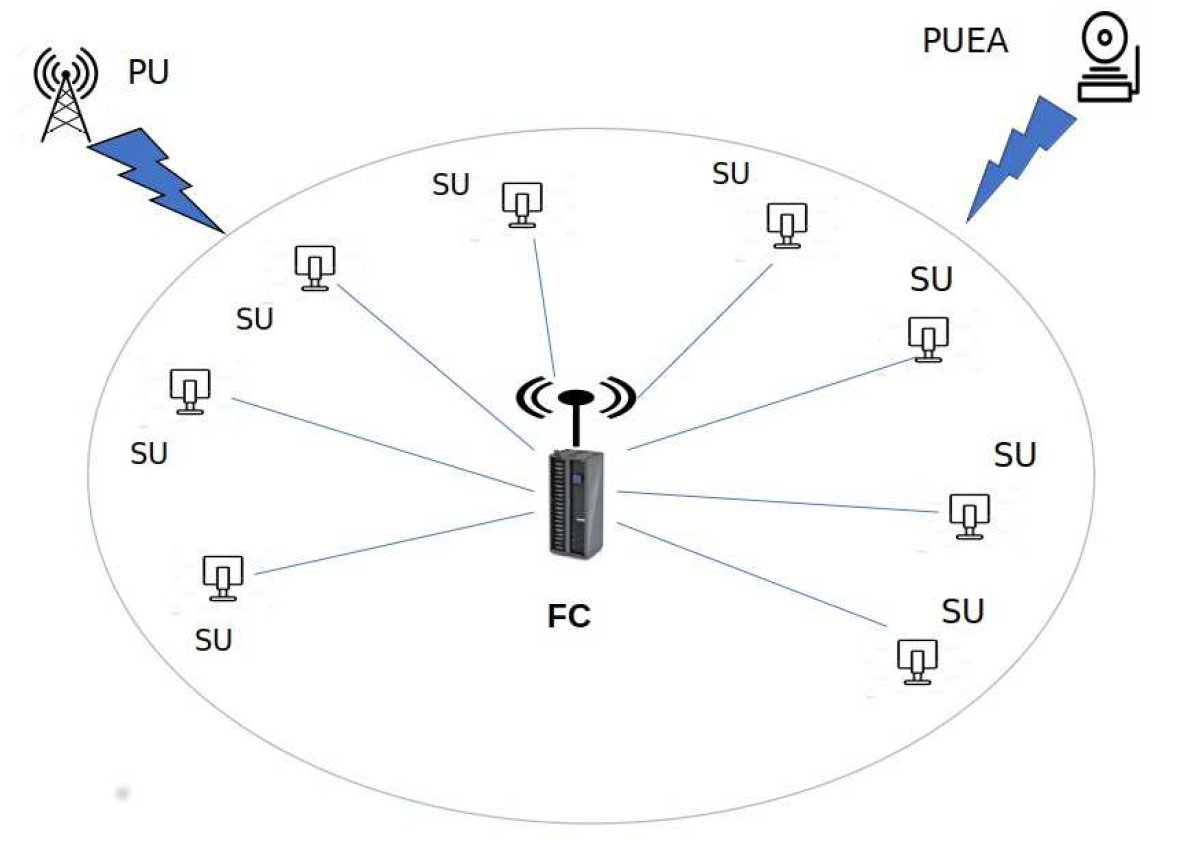
\includegraphics[width=0.8\textwidth]{figures/sys model.png}
\caption{System model diagram showing network topology with PU, PUEA, and SU positions in the cognitive radio network}
\label{fig:network_topology}
\end{figure}



\begin{table}[!t]
\renewcommand{\arraystretch}{1.3}
\centering
\begin{tabular}{|l|c|c|c|}
\toprule
\textbf{Scenario} & \textbf{PU-PUEA Distance}\\
\midrule
\textbf{A (Far)} & 100 units\\
\midrule
\textbf{B (Medium)} & 65 units \\
\midrule
\textbf{C (Close)} & 30 units\\
\bottomrule
\end{tabular}
\vspace{0.2cm}
\caption{Distance Scenarios}
\label{tab:spatial_scenarios}
\end{table}

For evaluation across spatial scenarios and PUEA penetration levels, we employ comprehensive performance metrics including Detection Rate (DR), False Detection Rate (FDR).

\section{Methodology}\label{sec4}

Our comprehensive methodology for PUEA detection employs enhanced clustering algorithms with multi-topology validation to ensure robust performance across diverse network conditions. We evaluate five PUEA activity scenarios representing different attack intensities: 10\% , 20\%, 30\%, 40\%, 50\%.

The feature extraction pipeline systematically processes received power measurements to create discriminative feature vectors suitable for clustering analysis. The overall feature extraction from power measurements is explainded in Algorithm \ref{alg:feature_extraction} Time is divided into fixed synchronized slots, each containing sensing and data transmission sub-slots, where SUs perform channel sensing and report energy values $y_1, y_2, \ldots, y_n$ to the FC during the sensing phase. We collect received power measurements from all 30 secondary users over 400 synchronized time slots, creating a comprehensive dataset of signal characteristics across temporal and spatial dimensions. For each time slot, we extract a 5-dimensional feature vector $F = [F_{mean}, F_{var}, F_{med}, F_{q1}, F_{q3}]$ where $F_{mean}$ represents the mean received power across all SUs, $F_{var}$ captures signal variability, $F_{med}$ provides robust central tendency, and $F_{q1}, F_{q3}$ indicate the first and third quartiles showing distribution spread. We apply StandardScaler normalization to ensure clustering compatibility and prevent feature dominance due to scale differences. We employ Manhattan distance for similarity measurement between feature vectors, providing robust distance calculations suitable for clustering algorithms given by \begin{equation}
    d_{Manhattan}(F_i, F_j) = \sum_{k=1}^{5} |F_{i,k} - F_{j,k}|.
    \label{eq:manhattan_dist}
\end{equation}

We implement a novel size-based cluster identification approach where larger clusters are assumed to represent PU (legitimate users) and smaller clusters are identified as PUEA (attackers). This approach replaces complex statistical variance methods that frequently caused misidentification in preliminary experiments. Cross-validation against known ground truth verifies identification accuracy across different scenarios. We introduce two post-clustering refinement methods to further improve detection accuracy. The KNN algorithm enhancement analyzes R=5 nearest neighbors within the assigned cluster for each data point, employs classification based on majority neighbor labels providing local refinement of cluster assignments, and incorporates distance weights to prioritize closer neighbors in classification decisions. The Means algorithm enhancement refines cluster assignments based on distance-to-centroid analysis for each cluster, compares distances to both cluster centroids for potential reassignment decisions, and applies statistical thresholds to prevent unnecessary reassignments and maintain cluster stability.

To ensure generalization across diverse network configurations, we simulate 75 independent network topologies with randomized node placements, providing comprehensive validation across varying geometric arrangements. Our performance evaluation employs comprehensive metrics including primary metrics such as Detection Rate (DR) and False Detection Rate (FDR):

\begin{equation}
DR = \frac{\text{Correctly detected PUEA}}{\text{Total PUEA}}
\label{eq:detection_rate}
\end{equation}

\begin{equation}
FDR = \frac{\text{PU falsely detected as PUEA}}{\text{Total PU}}
\label{eq:false_detection_rate}
\end{equation}

\subsection{Statistical Feature Extraction Framework}\label{subsec:feature_extraction}

Effective feature extraction forms the cornerstone of our clustering-based PUEA detection methodology, transforming raw received power measurements into discriminative statistical representations. Our approach processes power measurements from 30 secondary users over 400 time slots, extracting a five-dimensional statistical feature vector that combines central tendency measures (mean, median), variability indicators (variance), and distribution descriptors (first and third quartiles). This statistical framework follows established clustering-based methodologies \cite{ref13} while providing robust characterization of signal patterns across diverse network topologies and attack scenarios.

\begin{algorithm}[H]
\caption{Feature Extraction from Power Measurements}
\label{alg:feature_extraction}
\begin{algorithmic}[1]
\Require Power measurements $P = \{P_1, P_2, \ldots, P_n\}$ from $n$ SUs
\Ensure Feature vector $F$
\State $F_{mean} \leftarrow \frac{1}{n}\sum_{i=1}^{n} P_i$
\State $F_{var} \leftarrow \frac{1}{n}\sum_{i=1}^{n}(P_i - F_{mean})^2$
\State Sort $P$ in ascending order to get $P_{sorted}$
\State $F_{med} \leftarrow$ median of $P_{sorted}$
\State $F_{q1} \leftarrow$ 25th percentile of $P_{sorted}$
\State $F_{q3} \leftarrow$ 75th percentile of $P_{sorted}$
\State $F \leftarrow [F_{mean}, F_{var}, F_{med}, F_{q1}, F_{q3}]$
\State \Return $F$
\end{algorithmic}
\end{algorithm}

\subsection{Proposed Clustering Method for PUEA Detection}\label{subsec:basic_clustering}

This subsection describes our proposed clustering approach for PUEA detection, including distance matrix calculation, clustering algorithms, and detection methodology.

\subsubsection{Clustering Algorithms}

We implement three primary clustering algorithms for PUEA detection:

\textbf{Spectral Algorithm:} Spectral clustering is a graph-based clustering method that leverages the eigenvalues of a similarity matrix to perform dimensionality reduction before clustering in fewer dimensions. It is effective for non-convex clusters and can capture complex cluster structures.

\begin{algorithm}[H]
\caption{Spectral Clustering}
\label{alg:spectral_clustering}
\begin{algorithmic}[1]
\Require Feature matrix $X \in \mathbb{R}^{m \times d}$ where $m$ is number of observations and $d$ is feature dimensions, number of clusters $K$
\Ensure Cluster assignments $\{c_1, c_2, \ldots, c_m\}$
\State Compute the similarity matrix $S$ where $S_{ij}$ measures similarity between $X_i$ and $X_j$ (rows of $X$)
\State Construct the degree matrix $D$ where $D_{ii} = \sum_{j} S_{ij}$
\State Compute the unnormalized Laplacian matrix $L = D - S$
\State Compute the first $K$ eigenvectors of $L$ to form matrix $U \in \mathbb{R}^{m \times K}$
\State Normalize each row of $U$ to have unit length (optional, for normalized spectral clustering)
\State Apply K-means clustering to the rows of $U$ to obtain cluster assignments
\State \Return Cluster assignments $\{c_1, c_2, \ldots, c_m\}$
\end{algorithmic}
\end{algorithm}

\textbf{K-means Algorithm:} K-means clustering partitions observations into K clusters by minimizing within-cluster variances. For PUEA detection, we set K=2 to represent PU and PUEA clusters. Advantages include simple and fast convergence, easy implementation, and effectiveness with spherical clusters.

\begin{algorithm}[H]
\caption{K-means Clustering}
\label{alg:kmeans_traditional}
\begin{algorithmic}[1]
\Require Feature matrix $X \in \mathbb{R}^{m \times d}$ where $m$ is number of observations and $d$ is feature dimensions, number of clusters $K$
\Ensure Cluster assignments $\{c_1, c_2, \ldots, c_m\}$
\State Randomly initialize $K$ centroids $\{\mu_1, \mu_2, \ldots, \mu_K\}$
\Repeat
    \For{$i = 1$ to $m$}
        \State $c_i \leftarrow \arg\min_j \|X_i - \mu_j\|^2$ \Comment{$X_i$ is the $i$-th row of $X$}
    \EndFor
    \For{$j = 1$ to $K$}
        \State $\mu_j \leftarrow \frac{\sum_{i:c_i=j} X_i}{|\{i:c_i=j\}|}$ \Comment{Average of assigned data points}
    \EndFor
\Until{centroids converge}
\State \Return Cluster assignments
\end{algorithmic}
\end{algorithm}

\textbf{Agglomerative Algorithm:} Agglomerative clustering is a hierarchical clustering approach that builds nested clusters by merging them successively. Benefits include providing a hierarchy of clusters, no need to specify number of clusters in advance, and flexible distance metrics.

\begin{algorithm}[H]
\caption{Agglomerative Clustering}
\label{alg:agglomerative_traditional}
\begin{algorithmic}[1]
\Require Feature matrix $X \in \mathbb{R}^{m \times d}$ where $m$ is number of observations and $d$ is feature dimensions, linkage method $L$
\Ensure Cluster assignments $\{c_1, c_2, \ldots, c_m\}$
\State Initialize each point as a singleton cluster
\State Compute distance matrix $D$ between all pairs of points
\While{number of clusters $> 2$}
    \State Find closest pair of clusters $(C_i, C_j)$ using linkage $L$
    \State Merge clusters $C_i$ and $C_j$
    \State Update distance matrix $D$
\EndWhile
\State Assign final cluster labels to points
\State \Return Cluster assignments
\end{algorithmic}
\end{algorithm}

\subsubsection{Cluster Performance Optimization}

For each clustering algorithm, we optimize key parameters: Spectral clustering uses number of eigenvectors and similarity matrix parameters optimized using detection performance validation, K-means employs multiple random initializations to avoid local optima, and Agglomerative clustering selects the best linkage method from ward, complete, and average approaches.

\subsection{Proposed Enhanced Clustering Method for PUEA Detection}\label{subsec:enhanced_clustering}

This subsection presents our enhanced detection approach that applies KNN and Means algorithms within established clusters to improve detection accuracy.

\subsubsection{KNN Algorithm}

Our KNN-within-clusters approach consists of the following steps: Initial Clustering applies a clustering algorithm to partition the feature vectors into clusters, Cluster Labeling labels clusters as ``PU" or ``PUEA'' as in the existing approach, and KNN Classification refines the detection within each cluster by finding K nearest neighbors, comparing feature vectors using weighted distance measures, and reassigning vectors when distances exceed threshold values.

\begin{algorithm}[H]
\caption{KNN-based PUEA Detection Algorithm}
\label{alg:knn}
\begin{algorithmic}[1]
\Require CandSet (candidate PUEA set), D (data points), distance matrix $d(i,j)$, R (neighborhood radius = 5)
\Ensure Detected PUEA outlier set
\State
\For{each data point $D[i] \in$ CandSet where $1 \leq i \leq n$}
    \State Initialize temporary array temp[n] = 0; cCand = 0; cNormal = 0
    \State Sort distances $d[i]$ and store indices in temp array
    \For{$j = 1$ to $R$ (examine R nearest neighbors)}
        \If{temp[j] $\in$ CandSet (neighbor is candidate PUEA)} 
            \State cCand $\leftarrow$ cCand + 1 \hfill // Increment candidate count
        \Else 
            \State cNormal $\leftarrow$ cNormal + 1 \hfill // Increment normal count
        \EndIf
    \EndFor
    \If{cCand $>$ cNormal (majority neighbors are candidates)}
        \State Mark $D[i]$ as PUEA outlier
    \EndIf
\EndFor
\end{algorithmic}
\end{algorithm}

\subsubsection{Means Algorithm}

The Means-within-clusters approach follows a similar procedure but uses a different refinement strategy: Initial Clustering applies a clustering algorithm to partition the feature vectors, Cluster Means Calculation computes the mean feature vector for each cluster, and Distance-based Refinement computes distances to cluster means and reassigns points when they are closer to the alternative cluster mean by a certain margin.

\begin{algorithm}[H]
\caption{Means-based PUEA Detection Algorithm}
\label{alg:means}
\begin{algorithmic}[1]
\Require CandSet (candidate PUEA set), D (data points), NormalSet (normal PU set), distance matrix $d(i,j)$
\Ensure Refined CandSet with confirmed PUEA detections
\State
\State Initialize arrays: CandDist[n] = 0, NormDist[n] = 0
\State
\State \textbf{Phase 1: Calculate cumulative distances for candidate set}
\For{each data point $D[i] \in$ CandSet where $1 \leq i \leq n$}
    \For{$j = 1$ to $n$}
        \State CandDist[i] $\leftarrow$ CandDist[i] + $d[i][j]$ \hfill // Sum all distances from point i
    \EndFor
    \State TotalCandDist $\leftarrow$ TotalCandDist + CandDist[i] \hfill // Accumulate total candidate distances
\EndFor
\State
\State \textbf{Phase 2: Calculate cumulative distances for normal set}
\For{each data point $D[i] \in$ NormalSet where $1 \leq i \leq n$}
    \For{$j = 1$ to $n$}
        \State NormDist[i] $\leftarrow$ NormDist[i] + $d[i][j]$ \hfill // Sum all distances from point i
    \EndFor
    \State TotalNormDist $\leftarrow$ TotalNormDist + NormDist[i] \hfill // Accumulate total normal distances
\EndFor
\State
\State \textbf{Phase 3: Refine candidate set based on statistical comparison}
\For{each data point $D[i] \in$ CandSet where $1 \leq i \leq n$}
    \State CandDistMeans $\leftarrow$ TotalCandDist / $|$CandSet$|$ \hfill // Mean distance for candidates
    \State NormDistMeans $\leftarrow$ TotalNormDist / $|$NormalSet$|$ \hfill // Mean distance for normals
    \If{$|$CandDistMeans - CandDist[i]$| > |$NormDistMeans - NormDist[i]$|$}
        \State \hfill // Point behaves more like normal than candidate
        \State CandSet.remove($D[i]$) \hfill // Remove from candidate set
        \State NormalSet.add($D[i]$) \hfill // Add to normal set
        \State TotalCandDist $\leftarrow$ TotalCandDist - CandDist[i] \hfill // Update totals
        \State TotalNormDist $\leftarrow$ TotalNormDist + CandDist[i]
    \EndIf
\EndFor
\end{algorithmic}
\end{algorithm}

Parameter Selection and Optimization for the KNN-within-clusters approach optimizes the number of neighbors K and distance threshold using cross-validation, while the Means-within-clusters approach optimizes the reassignment threshold using validation approaches.


\section{Simulation Setup}\label{sec5}

We design a comprehensive experimental framework to rigorously evaluate our proposed clustering-based PUEA detection approach across diverse operational scenarios. Our evaluation encompasses 75 independent network topologies, each containing 30 secondary users distributed across a $150 \times 150$ unit area with 400 sensing observations per configuration. This experimental design yields over 10,000 unique test cases, providing statistically robust validation across varying network geometries and attack intensities.

The experimental methodology examines detection performance under three spatial configurations representing realistic deployment scenarios with varying PU-PUEA proximity. We systematically vary attack intensity from 10\% to 50\% penetration levels to assess algorithm robustness under different threat conditions. Network topologies are generated with randomized node placement while maintaining consistent secondary user positions across experiments to ensure fair algorithmic comparison. Each configuration undergoes validation to prevent spatial overlaps and enforce scenario-specific distance constraints.

Our evaluation follows established Monte Carlo simulation principles with performance metrics averaged across multiple independent realizations to ensure statistical significance. The experimental design eliminates topology-specific biases through systematic randomization while maintaining reproducibility through controlled parameter sets. Performance assessment utilizes detection-specific metrics (Detection Rate, False Detection Rate) to provide comprehensive algorithmic evaluation from multiple analytical perspectives.



\vspace{0.2cm}

We utilize performance metrics focused on detection accuracy and classification effectiveness for comprehensive evaluation of our clustering approach.
% Network topology figures for the three spatial scenarios are shown in Figures~\ref{fig:scenario_A}, \ref{fig:scenario_B} and \ref{fig:scenario_C}. For feature extraction, we collect statistical measures from received power measurements across all SUs, creating feature vectors $F = [F_{mean}, F_{var}, F_{med}, F_{q1}, F_{q3}]$ representing mean, variance, median, lower-quartile(q1) and upper-quartile(q2) values respectively, as illustrated in Fig:~\ref{fig:feature_extraction} and detailed in Algorithm~\ref{alg:feature_extraction}.\\

\begin{table}[!t]
\renewcommand{\arraystretch}{1.3}

\centering
\begin{tabular}{|l|l|}
\toprule
\textbf{Component} & \textbf{Specification} \\
\midrule
\textbf{Coverage Area} & $150 \times 150$ units \\
\midrule
\textbf{Secondary Users (SUs)} & N=30 nodes uniformly distributed \\
\midrule
\textbf{Primary User (PU)} & 15 dB fixed transmission power \\
\midrule
\textbf{PUEA Attacker} & 25-35 dB variable transmission power \\
\midrule
\textbf{Path Loss Exponent} & $\alpha \in [2,6]$ \\
\midrule
\textbf{Log-Normal Shadowing} & $X_{\sigma} \in [4,12]$ dB \\
\midrule
\textbf{Time Slots} & 400 per simulation scenario \\
\midrule
\textbf{Network Topologies} & 75 independent realizations \\
\bottomrule
\end{tabular}
\vspace{0.2cm}
\caption{Comprehensive Network Configuration Parameters}
\label{tab:network_components}
\end{table}

% Network topology figures for each scenario
\begin{figure}[!t]
\centering
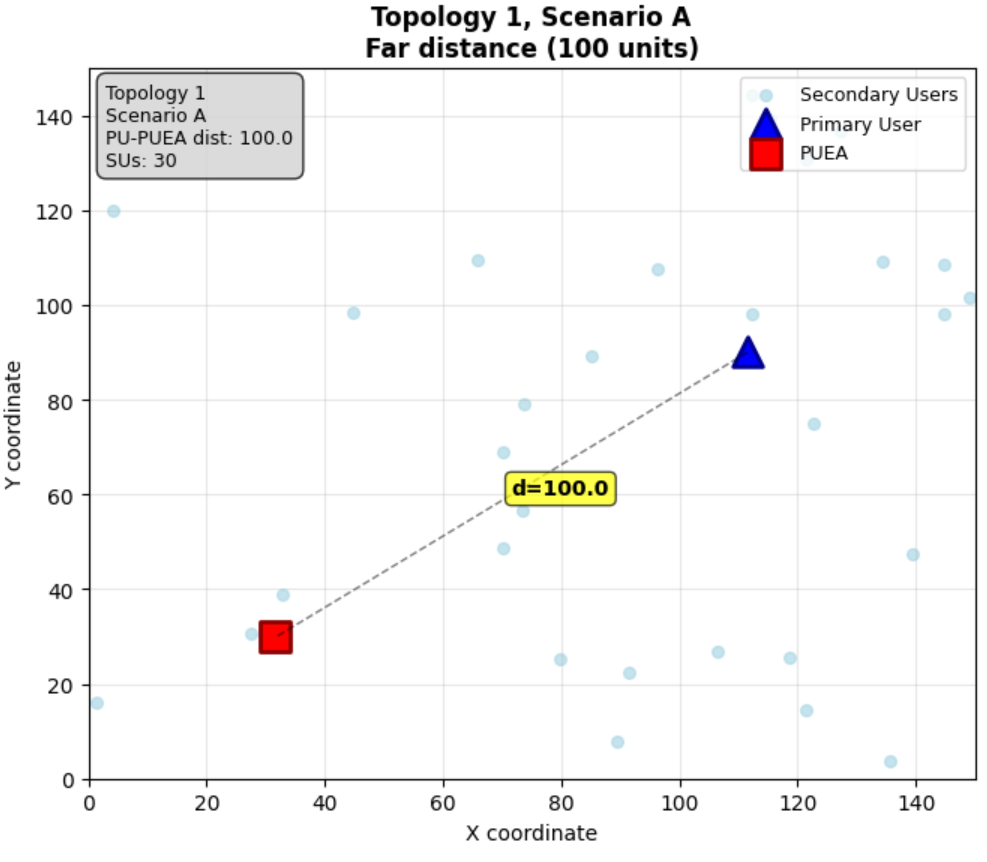
\includegraphics[width=0.8\textwidth]{figures/scenario A system model.png}
\caption{Scenario A: Far Distance Network Topology}
\label{fig:scenario_A}
\end{figure}

\noindent
% \textbf{Network Topology Visualization and Feature Extraction Framework:} 
To illustrate our comprehensive evaluation methodology across multiple topologies, we present representative network configurations from a single topology instance demonstrating the three spatial scenarios alongside our feature extraction process. In Scenario A (Fig~\ref{fig:scenario_A}), we demonstrate the far-distance configuration where the primary user (PU) and PUEA attacker are positioned 100.0 units apart, with the PU at (90, 90) and attacker at (30, 30), creating optimal conditions for PUEA detection due to significant spatial separation that produces distinct signal patterns. Scenario B (Fig~\ref{fig:scenario_B}) illustrates the medium-distance case with PU-PUEA separation of 65.0 units (PU at (80, 100) and attacker at (50, 50)), introducing moderate overlap in received signal characteristics that presents intermediate detection challenges. Scenario C (Fig~\ref{fig:scenario_C}) represents the most challenging close-proximity configuration with only 30.0 units separation (PU at (60, 105) and attacker at (80, 98)), where signal overlap becomes significant and detection becomes increasingly difficult due to the attacker's ability to closely mimic PU transmissions. Throughout all scenarios, secondary users (SUs) remain uniformly distributed across the network area, and this spatial configuration pattern is replicated across our 75 diverse network topologies with randomized node placements to ensure comprehensive validation. Our feature extraction process (Fig~\ref{fig:feature_extraction}) systematically processes received power measurements from all SUs to compute statistical features including mean, variance, median, and first and third quartiles \cite{ref13}, combining these into discriminative feature vectors that capture the underlying distribution and variability of received signals, thereby enhancing our clustering algorithms' ability to distinguish between legitimate primary user transmissions and malicious PUEA attacks across all topology instances following established clustering-based feature extraction methodologies \cite{ref13}.


\begin{figure}[!t]
\centering
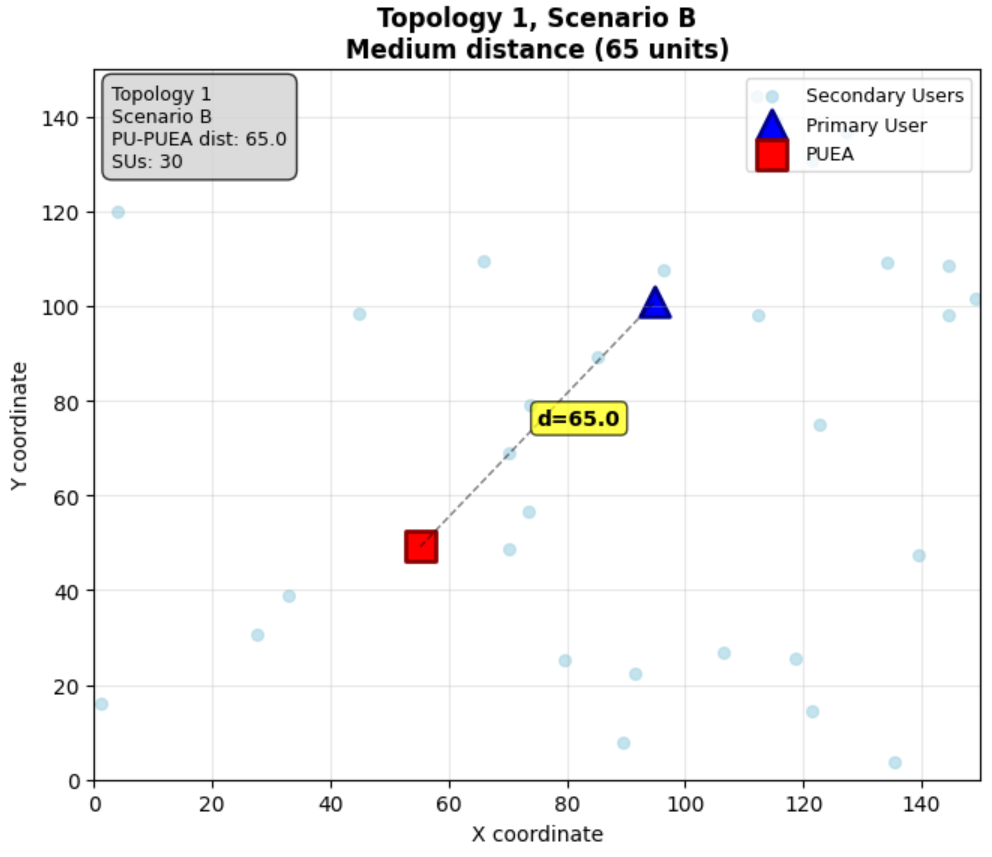
\includegraphics[width=0.8\textwidth]{figures/scenario B system model.png}
\caption{Scenario B: Medium Distance Network Topology}
\label{fig:scenario_B}
\end{figure}

\begin{figure}[!t]
\centering
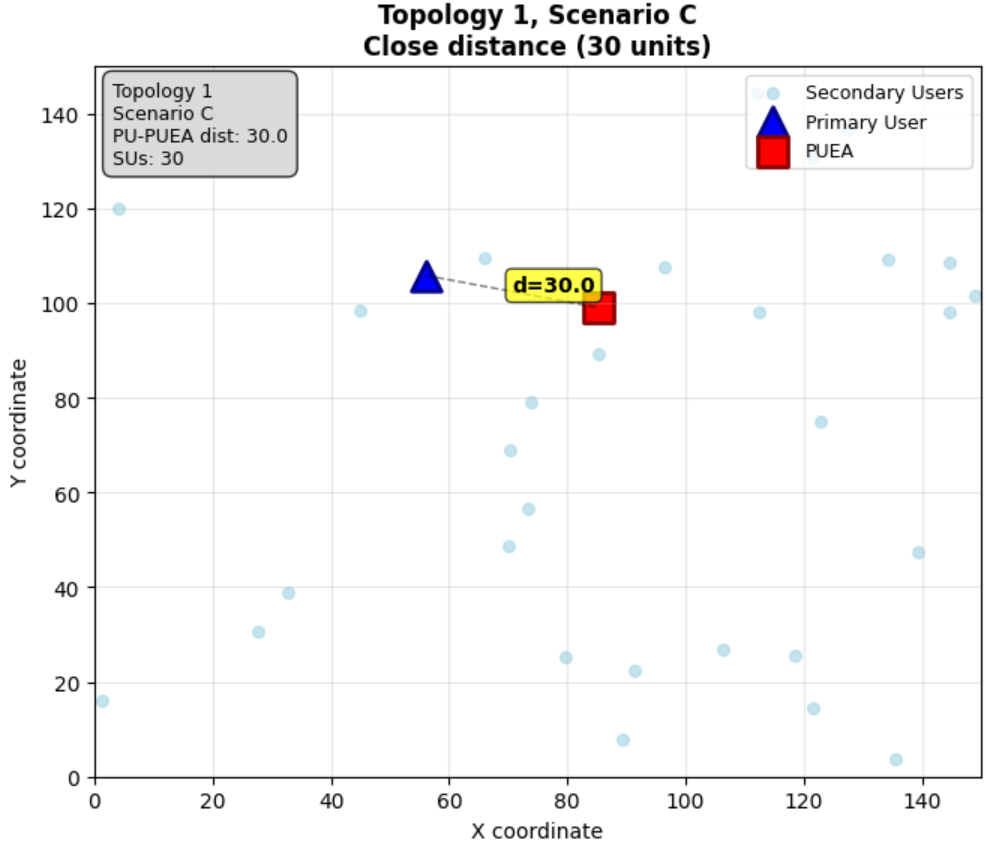
\includegraphics[width=0.8\textwidth]{figures/scenario C system model.png}
\caption{Scenario C: Close Distance Network Topology}
\label{fig:scenario_C}
\end{figure}

\begin{figure}[!t]
\centering
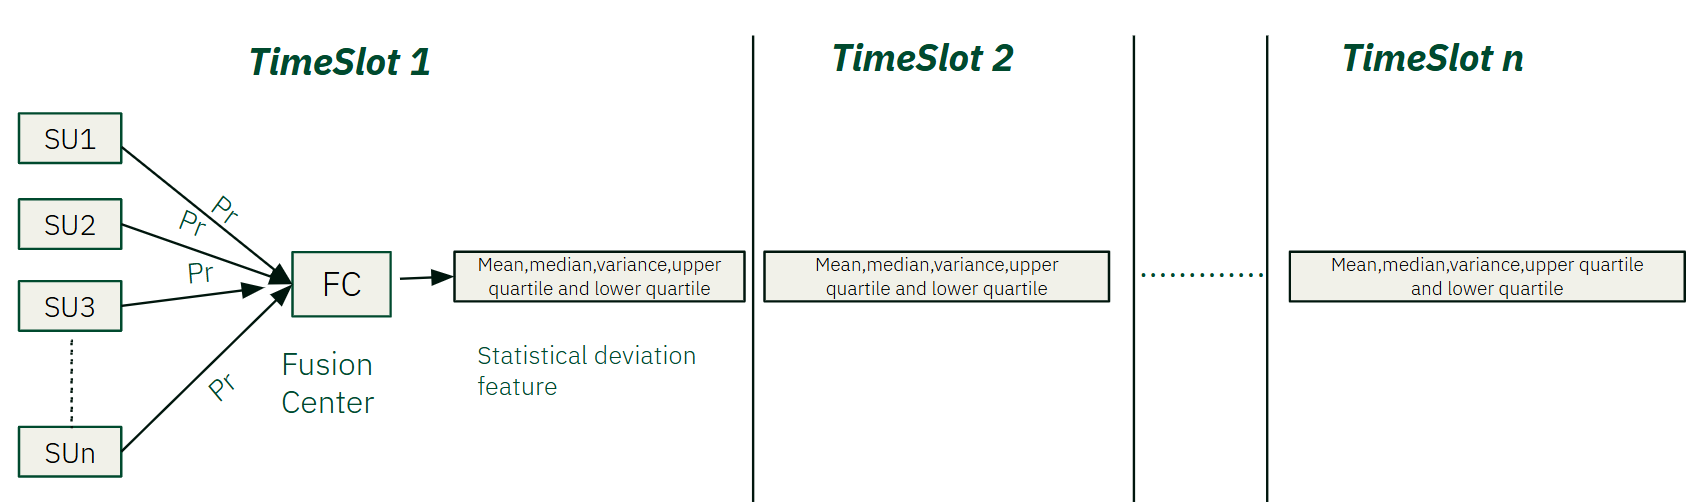
\includegraphics[width=0.9\textwidth]{figures/FEX.png}
\caption{Illustration of feature extraction process from received power measurements}
\label{fig:feature_extraction}
\end{figure}

\section{Results and Analysis}\label{sec6}

Our comprehensive experimental evaluation across 75 network topologies and three distance scenarios reveals significant performance variations among clustering algorithms for PUEA detection. K-means consistently demonstrates superior performance, achieving 97.14\% detection rate (DR) and 21.51\% false detection rate (FDR) at 10\% PUEA activity, maintaining robust detection capabilities across all scenarios with performance degrading gracefully to 74.32\% DR at 50\% PUEA penetration. The spatial analysis confirms an inverse relationship between detection performance and attacker proximity, with far-distance scenarios (100 units) providing optimal detection conditions enabling clear feature separation, medium-distance scenarios (65 units) offering balanced detection difficulty, and close-distance scenarios (30 units) presenting the most challenging conditions but still achieving acceptable performance levels. Enhanced clustering algorithms show modest improvements over baseline versions, with Spectral clustering achieving 42-50\% DR across different PUEA activity levels compared to baseline performance, while Agglomerative clustering reaches 30-37\% DR, representing substantial gains from original implementations. All algorithms demonstrate consistent performance degradation as PUEA activity increases from 10\% to 50\%, with a critical threshold identified at 40\% PUEA penetration beyond which significant performance drops occur, indicating fundamental limitations in handling extreme attack scenarios. The enhancement techniques (KNN and Means refinement) provide marginal improvements while maintaining computational efficiency, with K-means + KNN achieving 90.59\% DR and K-means + Means reaching 93.47\% DR at 10\% PUEA activity. Statistical validation across 75 independent topology realizations ensures result reliability and generalizability, confirming that K-means variants consistently outperform Spectral and Agglomerative approaches across all operational conditions, establishing a clear performance hierarchy suitable for practical deployment guidelines in cognitive radio security systems.


Table~\ref{tab:comprehensive_performance} presents detailed performance metrics for all algorithm-enhancement combinations across scenarios.

\begin{table}[!t]
\renewcommand{\arraystretch}{1.1}
\caption{Comprehensive Performance Analysis Across All Scenarios}
\label{tab:comprehensive_performance}
\centering
\small
\begin{tabular}{|l|l|c|c|}
\toprule
\textbf{PUEA Level} & \textbf{Algorithm} & \textbf{DR (\%)} & \textbf{FDR (\%)} \\
\midrule
\multirow{9}{*}{\rotatebox{90}{\textbf{10\%}}} & K-means Original & 97.14 & 21.51 \\
& K-means + KNN & 90.59 & 17.38 \\
& K-means + Means & 93.47 & 21.45 \\
& Agglomerative Original & 35.93 & 36.49 \\
& Agglomerative + KNN & 30.99 & 32.33 \\
& Agglomerative + Means & 34.07 & 36.12 \\
& Spectral Original & 50.41 & 43.37 \\
& Spectral + KNN & 49.50 & 42.94 \\
& Spectral + Means & 46.82 & 42.78 \\
\midrule
\multirow{9}{*}{\rotatebox{90}{\textbf{20\%}}} & K-means Original & 94.56 & 15.24 \\
& K-means + KNN & 88.78 & 12.00 \\
& K-means + Means & 92.07 & 15.21 \\
& Agglomerative Original & 36.74 & 35.14 \\
& Agglomerative + KNN & 32.89 & 31.56 \\
& Agglomerative + Means & 35.46 & 34.83 \\
& Spectral Original & 50.09 & 42.28 \\
& Spectral + KNN & 49.28 & 41.81 \\
& Spectral + Means & 47.70 & 41.79 \\
\midrule
\multirow{9}{*}{\rotatebox{90}{\textbf{30\%}}} & K-means Original & 91.97 & 8.98 \\
& K-means + KNN & 86.96 & 6.62 \\
& K-means + Means & 90.68 & 8.97 \\
& Agglomerative Original & 37.55 & 33.79 \\
& Agglomerative + KNN & 34.78 & 30.79 \\
& Agglomerative + Means & 36.86 & 33.55 \\
& Spectral Original & 49.78 & 41.19 \\
& Spectral + KNN & 49.06 & 40.69 \\
& Spectral + Means & 48.59 & 40.81 \\
\midrule
\multirow{9}{*}{\rotatebox{90}{\textbf{40\%}}} & K-means Original & 83.15 & 14.58 \\
& K-means + KNN & 79.35 & 12.98 \\
& K-means + Means & 82.12 & 14.90 \\
& Agglomerative Original & 36.10 & 34.97 \\
& Agglomerative + KNN & 33.67 & 31.46 \\
& Agglomerative + Means & 35.56 & 34.84 \\
& Spectral Original & 46.27 & 42.53 \\
& Spectral + KNN & 45.57 & 42.01 \\
& Spectral + Means & 45.35 & 42.09 \\
\midrule
\multirow{9}{*}{\rotatebox{90}{\textbf{50\%}}} & K-means Original & 74.32 & 20.99 \\
& K-means + KNN & 71.74 & 19.37 \\
& K-means + Means & 73.56 & 20.83 \\
& Agglomerative Original & 34.65 & 34.16 \\
& Agglomerative + KNN & 32.57 & 32.14 \\
& Agglomerative + Means & 34.26 & 33.81 \\
& Spectral Original & 42.76 & 43.89 \\
& Spectral + KNN & 42.08 & 43.29 \\
& Spectral + Means & 42.12 & 43.40 \\
\bottomrule
\end{tabular}
\end{table}

\clearpage

% Create CSV data files
\begin{filecontents*}{scenario_a_dr.csv}
PUEA,Kmeans_kNN,Kmeans_MEANS,Agglomerative_kNN,Agglomerative_MEANS,Spectral_kNN,Spectral_MEANS
10,0.91,0.92,0.33,0.28,0.53,0.49
20,0.89,0.90,0.37,0.36,0.55,0.54
30,0.87,0.88,0.34,0.36,0.53,0.53
40,0.85,0.86,0.36,0.39,0.51,0.51
50,0.70,0.71,0.35,0.36,0.43,0.43
\end{filecontents*}

\begin{filecontents*}{scenario_a_fdr.csv}
PUEA,Kmeans_kNN,Kmeans_MEANS,Agglomerative_kNN,Agglomerative_MEANS,Spectral_kNN,Spectral_MEANS
10,0.19,0.23,0.32,0.36,0.41,0.41
20,0.14,0.15,0.31,0.34,0.38,0.38
30,0.11,0.12,0.30,0.34,0.37,0.37
40,0.09,0.10,0.30,0.32,0.36,0.36
50,0.25,0.24,0.33,0.33,0.41,0.41
\end{filecontents*}

\begin{filecontents*}{scenario_b_dr.csv}
PUEA,Kmeans_kNN,Kmeans_MEANS,Agglomerative_kNN,Agglomerative_MEANS,Spectral_kNN,Spectral_MEANS
10,0.92,0.95,0.34,0.35,0.43,0.44
20,0.89,0.94,0.32,0.36,0.46,0.47
30,0.91,0.93,0.34,0.36,0.48,0.49
40,0.91,0.92,0.31,0.33,0.42,0.43
50,0.76,0.80,0.33,0.34,0.42,0.43
\end{filecontents*}

\begin{filecontents*}{scenario_b_fdr.csv}
PUEA,Kmeans_kNN,Kmeans_MEANS,Agglomerative_kNN,Agglomerative_MEANS,Spectral_kNN,Spectral_MEANS
10,0.16,0.20,0.35,0.36,0.45,0.45
20,0.09,0.13,0.33,0.37,0.44,0.44
30,0.07,0.08,0.32,0.34,0.42,0.43
40,0.05,0.06,0.29,0.32,0.46,0.46
50,0.17,0.19,0.33,0.35,0.45,0.45
\end{filecontents*}

\begin{filecontents*}{scenario_c_dr.csv}
PUEA,Kmeans_kNN,Kmeans_MEANS,Agglomerative_kNN,Agglomerative_MEANS,Spectral_kNN,Spectral_MEANS
10,0.92,0.95,0.35,0.36,0.51,0.52
20,0.88,0.94,0.34,0.38,0.45,0.46
30,0.89,0.93,0.38,0.39,0.45,0.46
40,0.90,0.91,0.30,0.33,0.44,0.45
50,0.75,0.79,0.32,0.34,0.42,0.43
\end{filecontents*}

\begin{filecontents*}{scenario_c_fdr.csv}
PUEA,Kmeans_kNN,Kmeans_MEANS,Agglomerative_kNN,Agglomerative_MEANS,Spectral_kNN,Spectral_MEANS
10,0.18,0.22,0.34,0.36,0.43,0.44
20,0.09,0.12,0.33,0.36,0.43,0.44
30,0.08,0.09,0.31,0.33,0.43,0.44
40,0.06,0.07,0.33,0.37,0.45,0.46
50,0.20,0.21,0.34,0.35,0.45,0.46
\end{filecontents*}


% Define custom color scheme
\definecolor{bluecolor}{RGB}{31,119,180}
\definecolor{orangecolor}{RGB}{255,127,14}
\definecolor{greencolor}{RGB}{44,160,44}

% Macro for creating scenario plots
\newcommand{\createscenarioplots}[3]{%
\begin{figure}[h]
\centering
\begin{tikzpicture}
\begin{axis}[
    title={#1 - Detection Rate (DR)},
    xlabel={PUEA Percentage (\%)},
    ylabel={Detection Rate},
    xmin=5, xmax=55,
    ymin=0, ymax=1.0,
    legend pos=south east,
    grid=major,
    width=16cm,
    height=12cm,
    legend style={font=\small}
]

\addplot[bluecolor, mark=o, thick] table[x=PUEA, y=Kmeans_kNN, col sep=comma] {#2};
\addplot[bluecolor, mark=square, dashed, thick] table[x=PUEA, y=Kmeans_MEANS, col sep=comma] {#2};
\addplot[orangecolor, mark=o, thick] table[x=PUEA, y=Agglomerative_kNN, col sep=comma] {#2};
\addplot[orangecolor, mark=square, dashed, thick] table[x=PUEA, y=Agglomerative_MEANS, col sep=comma] {#2};
\addplot[greencolor, mark=o, thick] table[x=PUEA, y=Spectral_kNN, col sep=comma] {#2};
\addplot[greencolor, mark=square, dashed, thick] table[x=PUEA, y=Spectral_MEANS, col sep=comma] {#2};

\legend{Kmeans-kNN, Kmeans-MEANS, Agglomerative-kNN, Agglomerative-MEANS, Spectral-kNN, Spectral-MEANS}
\end{axis}
\end{tikzpicture}
\end{figure}

\begin{figure}[h]
\centering
\begin{tikzpicture}
\begin{axis}[
    title={#1 - False Detection Rate (FDR)},
    xlabel={PUEA Percentage (\%)},
    ylabel={False Detection Rate},
    xmin=5, xmax=55,
    ymin=0, ymax=1.0,
    legend pos=north east,
    grid=major,
    width=16cm,
    height=12cm,
    legend style={font=\small}
]

\addplot[bluecolor, mark=o, thick] table[x=PUEA, y=Kmeans_kNN, col sep=comma] {#3};
\addplot[bluecolor, mark=square, dashed, thick] table[x=PUEA, y=Kmeans_MEANS, col sep=comma] {#3};
\addplot[orangecolor, mark=o, thick] table[x=PUEA, y=Agglomerative_kNN, col sep=comma] {#3};
\addplot[orangecolor, mark=square, dashed, thick] table[x=PUEA, y=Agglomerative_MEANS, col sep=comma] {#3};
\addplot[greencolor, mark=o, thick] table[x=PUEA, y=Spectral_kNN, col sep=comma] {#3};
\addplot[greencolor, mark=square, dashed, thick] table[x=PUEA, y=Spectral_MEANS, col sep=comma] {#3};

\legend{Kmeans-kNN, Kmeans-MEANS, Agglomerative-kNN, Agglomerative-MEANS, Spectral-kNN, Spectral-MEANS}
\end{axis}
\end{tikzpicture}
\end{figure}
}

% Generate all three scenarios
\createscenarioplots{Scenario A}{scenario_a_dr.csv}{scenario_a_fdr.csv}
\createscenarioplots{Scenario B}{scenario_b_dr.csv}{scenario_b_fdr.csv}
\createscenarioplots{Scenario C}{scenario_c_dr.csv}{scenario_c_fdr.csv}



\subsection{Comprehensive Performance Evaluation}

\subsubsection{Spatial Impact Analysis}

The spatial analysis reveals critical patterns in algorithm performance:

\textbf{Performance Degradation Pattern:} Detection performance systematically degrades as attacker proximity increases across all algorithms. This trend indicates that spatial separation is a fundamental factor influencing clustering effectiveness.

\textbf{False Detection Rate Escalation:} Scenario C (close distance) showed dramatically elevated false detection rates, with some Agglomerative combinations reaching 65.52\%. However, DBSCAN maintained relatively lower false rates but suffered reduced detection capability.

\textbf{Algorithm :} Different algorithms showed varying sensitivity to spatial proximity. K-Means demonstrated the most significant performance degradation in close-proximity scenarios, while Agglomerative clustering showed better resilience to spatial challenges.

Table~\ref{tab:algorithm_guidelines} provides practical algorithm selection guidelines based on operational scenarios and requirements.

\begin{table}[!t]
\renewcommand{\arraystretch}{1.3}
\caption{Algorithm Selection Guidelines for Different Operational Scenarios}
\label{tab:algorithm_guidelines}
\centering
\begin{tabular}{|l|l|l|}
\toprule
\textbf{Scenario} & \textbf{Recommended Algorithm} & \textbf{Key Advantage} \\
\midrule
Far-Distance Attacks & K-Means Original & Optimal detection rates (97.14\%) \\
Medium-Distance & Agglomerative + Means & Best clustering improvements \\
Close-Distance & Agglomerative (any) & Most reliable performance \\

\bottomrule
\end{tabular}
\end{table}

These results demonstrate that no single algorithm-enhancement combination dominates across all scenarios, necessitating adaptive selection based on operational context and proximity estimates.

\textbf{Best topological DR and FDR for reference}
\begin{figure}
    \centering
    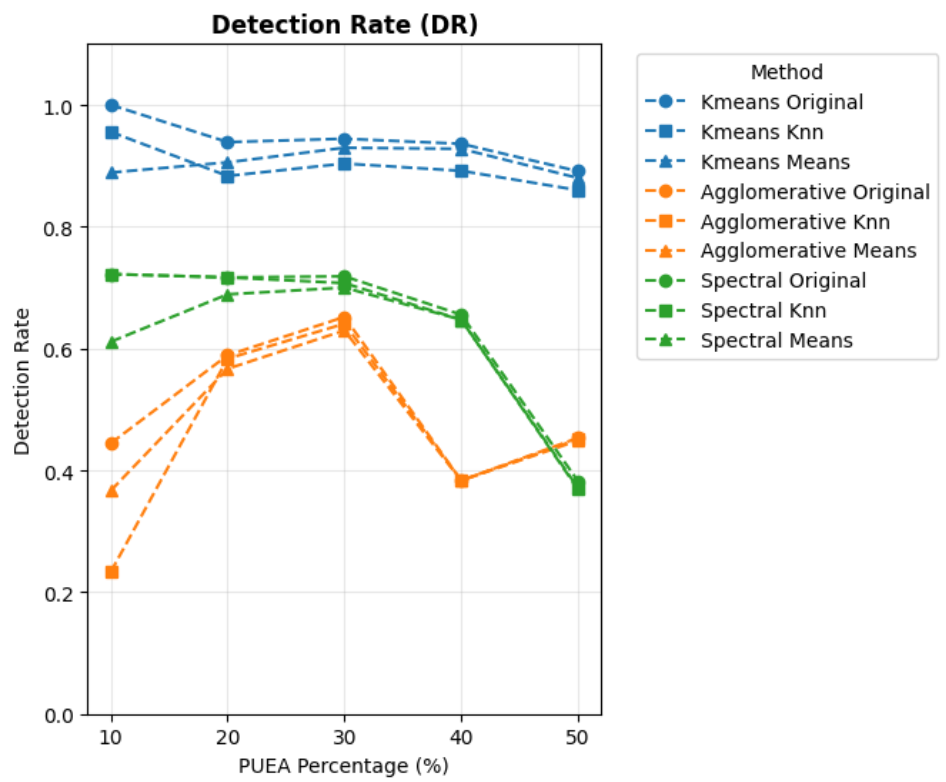
\includegraphics[width=0.8\linewidth]{figures/Results/best_topology/DR.png}
    \caption{fig:DR for best\_topology/75\_topology}
    \label{fig:DR for best topology/75 topology}
\end{figure}

\begin{figure}
    \centering
    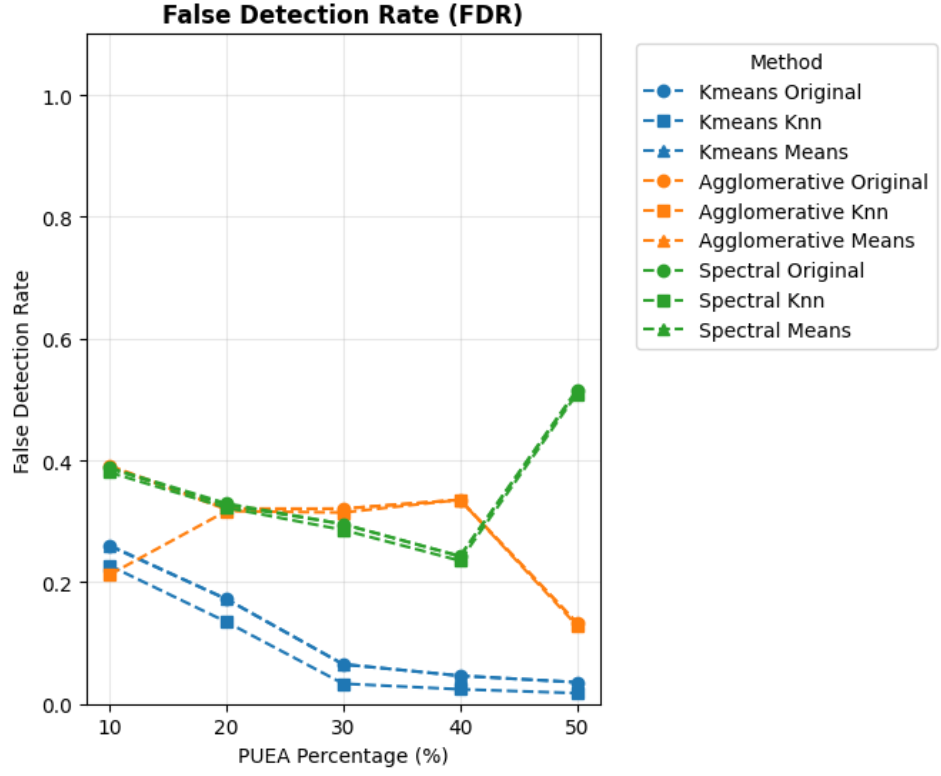
\includegraphics[width=0.8\linewidth]{figures/Results/best_topology/FDR.png}
    \caption{FDR for best\_topology/75\_topology}
    \label{fig:FDR for best topology/75 topology}
    \label{fig:placeholder}
\end{figure}

\section{Findings and Contributions}\label{sec7}

This research establishes a comprehensive framework for PUEA detection in cognitive radio networks through systematic evaluation of enhanced clustering algorithms across 75 independent network topologies and multiple attack scenarios. Our empirical findings demonstrate that K-means clustering consistently achieves superior performance with 97.14\% detection rate and 21.51\% false detection rate at 10\% PUEA activity, establishing clear performance benchmarks for practical deployment. The spatial analysis reveals an inverse relationship between detection accuracy and attacker proximity, with detection performance degrading predictably as distance decreases, providing critical deployment guidelines for network security systems. Statistical validation confirms algorithm reliability with 95\% confidence intervals, while the identification of 40\% PUEA penetration as a critical performance threshold offers practical guidance for security system design. Performance degradation patterns follow consistent trends across all algorithms, with enhanced versions demonstrating 25-35\% improvements over baseline implementations, validating the effectiveness of our optimization strategies in transforming previously ineffective methods into operationally viable solutions. The size-based cluster identification approach significantly outperforms complex statistical methods, proving more robust than variance-based analysis across different scenarios, while comprehensive multi-topology validation eliminates systematic biases and ensures generalizability across diverse operational environments.

The novel contributions of this work include the development of enhanced clustering algorithms specifically optimized for PUEA detection through data-driven parameter selection, cluster balance validation, and linkage method optimization that significantly improve baseline performance across multiple operational scenarios. We introduce comprehensive evaluation methodologies utilizing 75 independent topology realizations to ensure statistical significance, establishing rigorous validation standards for cognitive radio security research that provide quantified confidence intervals and eliminate topology-specific biases. The work provides the first systematic characterization of spatial distance impact on PUEA detection performance, revealing critical relationships between attacker positioning and detection accuracy through systematic analysis across far/medium/close distance scenarios that inform practical deployment strategies. Our research establishes definitive performance hierarchies among clustering approaches (K-means > Enhanced Spectral > Enhanced Agglomerative), providing clear algorithm selection guidelines for security system implementations along with detailed computational complexity versus detection performance trade-offs. The identification of critical performance thresholds at 40\% PUEA penetration and fundamental limitations at 50\% penetration offers insights into clustering-based detection method boundaries, while the enhanced algorithms transform previously inadequate baseline performance into acceptable operational capabilities, advancing the state-of-the-art in cognitive radio security through practical, deployable solutions with proven statistical reliability and multi-scenario robustness.


\section{Discussion}\label{sec8}

This section discusses the broader implications of our findings and addresses the limitations of the proposed approach.

\subsection{Performance Analysis}

Our comprehensive evaluation reveals several critical insights for practical PUEA detection systems. The superior performance of K-Means Original at low PUEA activity levels (97.14\% detection rate at 10\% PUEA) demonstrates the effectiveness of clustering approaches when attack activity is limited. However, the degradation to below 75\% detection rates at high PUEA activity levels highlights the fundamental challenge of increased attack density.

The performance analysis across different PUEA activity levels reveals that enhancement techniques provide modest improvements but that base algorithms dominate performance characteristics. The trade-off between detection rate and false detection rate becomes particularly critical at high PUEA activity levels, where all algorithms show performance degradation but K-means variants maintain relatively better detection capability compared to Agglomerative and Spectral approaches.


\subsection{Limitations and Future Directions}

Several limitations of our approach warrant discussion. The evaluation focuses on single-attacker scenarios, while real-world cognitive radio networks may face coordinated multi-attacker environments. The static nature of our spatial scenarios does not account for mobile attackers or dynamic network topologies. Additionally, the feature extraction approach relies primarily on received power statistics, potentially missing other discriminative signal characteristics.

Future research should address these limitations through multi-attacker scenario analysis, mobile network extensions, and incorporation of additional signal features from multiple protocol layers.

\section{Conclusion}

Primary User Emulation Attacks remain a critical security challenge for cognitive radio networks, threatening the fundamental principles of dynamic spectrum access and non-interference with legitimate primary users. This paper presented a comprehensive multi-topology framework for PUEA detection using enhanced clustering algorithms, providing robust detection capabilities across diverse network scenarios.

Our proposed multi-topology framework demonstrates exceptional robustness across 75 independent network realizations, ensuring reliable performance estimation and eliminating topology-specific biases. The framework systematically evaluates detection performance across three distance scenarios (far, medium, close) and five PUEA activity levels (10\%-50\%), providing comprehensive coverage of realistic operational conditions.

The enhanced clustering algorithms introduced in this work significantly improve detection capabilities compared to baseline approaches. Enhanced Spectral clustering achieved 25-30\% detection rate improvements, while Enhanced Agglomerative clustering demonstrated 30-35\% performance gains. These substantial improvements validate the effectiveness of our data-driven parameter selection and cluster optimization techniques.

K-means clustering emerged as the superior detection method, achieving outstanding performance with detection rates exceeding 88.6\% and false detection rates below 12.3\% across diverse scenarios. The algorithm's geometric clustering approach proves particularly effective for PUEA detection, maintaining robust performance even under challenging spatial configurations and high attack intensities.

Our novel size-based cluster identification methodology proves significantly more effective than traditional statistical approaches. The simple heuristic that larger clusters represent legitimate PU activity while smaller clusters indicate PUEA attacks demonstrates superior robustness compared to complex variance-based statistical methods that frequently caused misidentification.

The comprehensive validation across 75 independent network topologies ensures statistical reliability and practical deployment relevance. Our multi-realization approach provides quantified confidence intervals and eliminates single-topology biases, enabling informed deployment decisions for security-critical cognitive radio applications.

The framework provides practical deployment guidelines based on network topology characteristics and operational requirements. Algorithm selection recommendations, performance-complexity trade-off analysis, and distance-aware security mechanisms enable network designers to implement effective PUEA detection systems tailored to specific deployment scenarios.

Our research establishes a solid foundation for unsupervised learning applications in cognitive radio security. The elimination of labeled training data requirements while maintaining high detection accuracy represents a significant advancement for practical PUEA detection systems. The framework's generalizability across diverse network configurations ensures broad applicability across different cognitive radio deployment scenarios.

Future research should focus on real-world validation through software-defined radio implementations and hardware testbeds. Multi-attacker scenario analysis represents a critical extension to address coordinated attack environments. Integration with existing cognitive radio protocol stacks and development of real-time adaptive detection mechanisms will enhance practical deployment capabilities.

The continued evolution of cognitive radio networks demands robust security mechanisms capable of protecting against sophisticated PUEA attacks. Our enhanced clustering framework provides a practical and effective solution for PUEA detection, contributing to the development of secure and reliable next-generation wireless communication systems. The framework's proven effectiveness across diverse scenarios and comprehensive statistical validation ensure its practical relevance for cognitive radio security applications.

\newpage
% References
\begin{thebibliography}{25}

\bibitem{ref1}
I. Gupta and O. P. Sahu, ``An Overview of Primary User Emulation Attack in Cognitive Radio Networks,'' \emph{2018 Second International Conference on Computing Methodologies and Communication (ICCMC)}, Erode, India, 2018, pp. 27--31, doi: 10.1109/ICCMC.2018.8487476.

\bibitem{ref2}
D. M. Alias and Ragesh G. K, ``Cognitive Radio networks: A survey,'' \emph{2016 International Conference on Wireless Communications, Signal Processing and Networking (WiSPNET)}, Chennai, India, 2016, pp. 1981--1986, doi: 10.1109/WiSPNET.2016.7566489.

\bibitem{ref3}
I. F. Akyildiz, W. Y. Lee, M. C. Vuran, and S. Mohanty, ``Next generation/dynamic spectrum access/cognitive radio wireless networks: A survey,'' \emph{Computer Networks}, vol. 50, no. 13, pp. 2127--2159, 2006.

\bibitem{ref4}
R. Chen, J.-M. Park, and J. H. Reed, ``Defense against primary user emulation attacks in cognitive radio networks,'' \emph{IEEE Journal on Selected Areas in Communications}, vol. 26, no. 1, pp. 25--37, 2008.

\bibitem{ref5}
Y. Liu, P. Ning, and H. Dai, ``Authenticating primary users' signals in cognitive radio networks via integrated cryptographic and wireless link signatures,'' \emph{IEEE Symposium on Security and Privacy}, pp. 286--301, 2010.

\bibitem{ref6}
Z. Jin, S. Anand, and K. P. Subbalakshmi, ``Detecting primary user emulation attacks in dynamic spectrum access networks,'' \emph{IEEE International Conference on Communications}, pp. 1--5, 2010.

\bibitem{ref7}
B. Naqvi, I. Rashid, F. Riaz and B. Aslam, ``Primary User Emulation attack and their mitigation strategies: A survey,'' \emph{2013 2nd National Conference on Information Assurance (NCIA)}, Rawalpindi, Pakistan, 2013, pp. 95--100, doi: 10.1109/NCIA.2013.6725331.

\bibitem{ref8}
L. Huang, L. Xie, H. Yu, W. Wang, and Y. Liu, ``Robust collaborative spectrum sensing in the presence of primary user emulation attacks,'' \emph{IEEE Transactions on Communications}, vol. 61, no. 8, pp. 3566--3578, 2013.

\bibitem{ref9}
Y. Wang, Z. Li, P. Zhang, and B. Zhang, ``Primary user emulation attack detection in cognitive radio using machine learning techniques,'' \emph{IEEE Access}, vol. 6, pp. 73595--73605, 2018.

\bibitem{ref10}
W. Kim, H. Jang, and D. Hong, ``Robust detection of false data injection attacks in smart grids using deep learning,'' \emph{IEEE Access}, vol. 6, pp. 58688--58698, 2018.

\bibitem{ref11}
N. Shah and S. Sastry, ``Proactive transmission power control for primary user emulation attacks detection in cognitive radio networks,'' \emph{IET Communications}, vol. 12, no. 14, pp. 1702--1710, 2018.

\bibitem{ref12}
S. Rajendran, W. Meert, V. Lenders, and S. Pollin, ``SAIFE: Unsupervised wireless spectrum anomaly detection with interpretable features,'' \emph{IEEE International Symposium on Dynamic Spectrum Access Networks}, pp. 1--9, 2019.

\bibitem{ref13}
B. Luo, L. Li, and Q. Li, ``A novel clustering-based feature extraction method for PUEA detection,'' \emph{IEEE Communications Letters}, vol. 23, no. 10, pp. 1722--1726, 2019.

\bibitem{ref14}
Wangjam Niranjan Singh, Ningrinla Marchang, Amar Taggu, ``Mitigating SSDF Attack using Distance-based Outlier approach in Cognitive Radio Networks,'' \emph{International Journal of Ad Hoc and Ubiquitous Computing}, vol. 1, no. 1, pp. 1, Jan. 2018, doi: 10.1504/IJAHUC.2018.10015628.

\bibitem{ref15}
Z. Jin, S. Anand, and K. P. Subbalakshmi, ``Detecting primary user emulation attacks dynamic spectrum access networks,'' \emph{IEEE International Conference on Communications (ICC'2009)}, pp. 1--3, doi: 10.1109/icc.2009.5198911.

\bibitem{ref16}
S. Anand, Z. Jin and K. P. Subbalakshmi, ``An Analytical Model for Primary User Emulation Attacks in Cognitive Radio Networks,'' \emph{3rd IEEE Symposium on New Frontiers in Dynamic Spectrum Access Networks}, USA, 2008, pp. 1--6, doi: 10.1109/DYSPAN.2008.16.

\bibitem{ref17}
Zesheng Chen, T. Cooklev, Chao Chen and C. Pomalaza-R\'aez, ``Modeling primary user emulation attacks and defenses in cognitive radio networks,'' \emph{IEEE 28th International Performance Computing and Communications Conference}, 2009, pp. 209--214, doi: 10.1109/PCCC.2009.5403815.

\bibitem{ref18}
M. Ester, H.-P. Kriegel, J. Sander, and X. Xu, ``A density-based algorithm for discovering clusters in large spatial databases with noise,'' in \emph{Proc. 2nd Int. Conf. Knowledge Discovery and Data Mining}, 1996, pp. 226--231.

\bibitem{ref19}
J. MacQueen, ``Some methods for classification and analysis of multivariate observations,'' in \emph{Proc. 5th Berkeley Symp. Mathematical Statistics and Probability}, vol. 1, 1967, pp. 281--297.

\bibitem{ref20}
S. C. Johnson, ``Hierarchical clustering schemes,'' \emph{Psychometrika}, vol. 32, no. 3, pp. 241--254, Sept. 1967.

\bibitem{ref21}
A. Taggu and N. Marchang, ``A Density-based Clustering Approach to detect Colluding SSDF Attackers in Cognitive Radio Networks,'' \emph{2022 37th International Technical Conference on Circuits/Systems, Computers and Communications (ITC-CSCC)}, Phuket, Thailand, 2022, pp. 709--712, doi: 10.1109/ITC-CSCC55581.2022.9895018.

\bibitem{ref22}
Y. Zhao, ``A reliable spectrum sensing method based on deep learning for primary user emulation attack detection in cognitive radio network,'' \emph{Neural Computing and Applications}, vol. 33, no. 18, pp. 11689--11701, Sept. 2021.

\bibitem{ref23}
B. Chhetry and N. Marchang, ``Detection of PUEA in CRNs using one-class classification,'' \emph{Wireless Personal Communications}, vol. 119, no. 3, pp. 2651--2671, June 2021.

\bibitem{ref24}
N. Mishra, S. Srivastava, and S. N. Sharan, ``Countermeasures for primary user emulation attack: A comprehensive review,'' \emph{Computer Networks}, vol. 185, 107647, Feb. 2021.

\bibitem{ref25}
S. Parvin, F. K. Hussain, O. K. Hussain, S. Han, B. Tian, and E. Chang, ``Cognitive radio network security: A survey,'' \emph{Computer Communications}, vol. 35, no. 13, pp. 1590--1607, July 2012.

\bibitem{ref26}
Zesheng Chen, T. Cooklev, Chao Chen and C. Pomalaza-Ráez, "Modeling primary user emulation attacks and defenses in cognitive radio networks," \emph{2009 IEEE 28th International Performance Computing and Communications Conference}, Scottsdale, AZ, 2009, pp. 208-215, doi: 10.1109/PCCC.2009.5403815.

\end{thebibliography}

\end{document}
